\subsection{CajaMar Models}
\label{Section:CajaMarModels}

\subsubsection*{Introduction}


\subsubsection*{Model Structure}

From a probabilistic modeling point of view, Caja-Mar faces two different problems [][]: the prediction of the risk of defaulting of a customer in the next two years; and the extraction of profiles of ``desirable'' prospective customers. 

The risk prediction problem has been modeled as supervised dynamic prediction problem.  We are given a data base with a set of variables or predictors (some of them manually built by CajaMar's experts) describing the financial behavior of the customers and, also, whether the customer is considered as defaulter and non defaulter according to CajaMar standards (i.e. a binary class variable). The dynamic component of the problem needs to be considered because the behavior of the customers evolves over time (e.g. the account balance is continuously changing from month to another, the level of incomes, etc.)  as well as the labeling as defaulter or non-defaulter customer (e.g. one customer can be creditworthy and, but after some time, be in bankrupt for becoming unemployed). More specifically, the proposed model is expected to answer the following question: which is the probability that this customer will  default in some of his/her loans in two years? And this prediction has to be made only using the customer's behavior in the last 180 days \footnote{This limit is imposed by the Bank of Spain.}.

The graphical structure of the dynamic probabilistic graphical model devised for this problem is given in Figure \ref{Figure:CajaMarModel1}.  The yellow square boxes ``Day -180'', ..., ``Day-1'' represents the temporal evolution of the predictor variables. The model only refers to 180 days because this is the imposed limit of days when making predictions. Similarly, the class variable ``default'' is assumed to evolve over time but with the relevant different that the default class sequence refers to a point in the time \textbf{two years later} than  the point in the time the daily predictor variables. 

\begin{figure}
\begin{center}
\caption{\label{Figure:CajaMarModel1}Caja Mar Temporal Model}
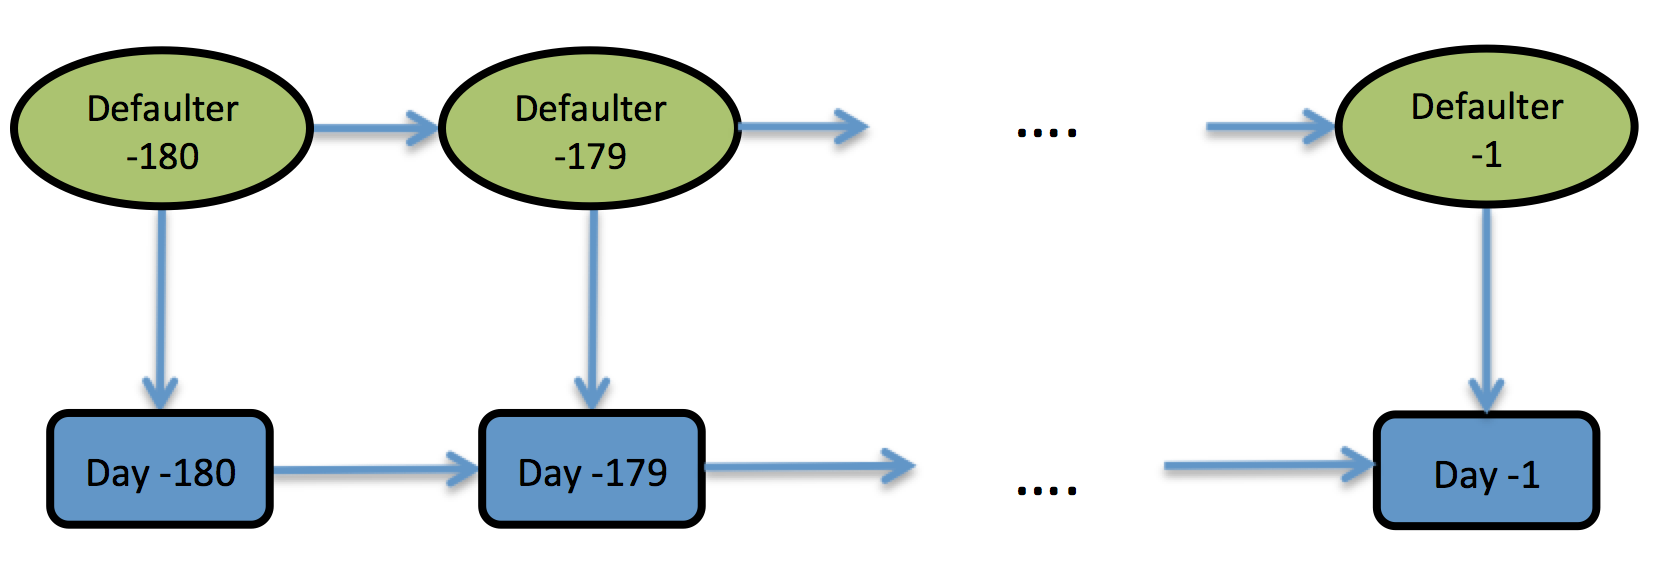
\includegraphics[scale=0.5]{./figures/CajaMarModel1}
\end{center}
\end{figure}


Finally, in Figure \ref{Figure:CajaMarModel2} we further detail the structure of the predictors variables evolving over time. 

\begin{figure}
\begin{center}
\caption{\label{Figure:CajaMarModel2} Basic component of the structure of the dynamic model}
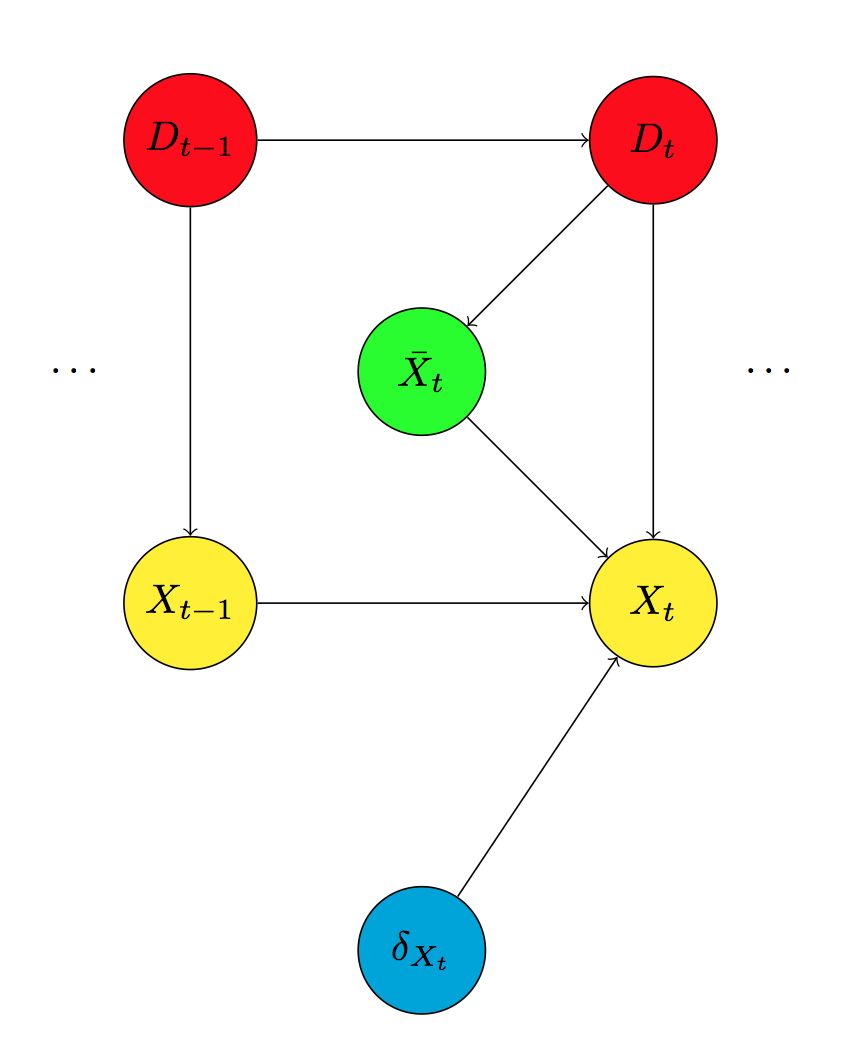
\includegraphics[scale=0.5]{./figures/CajaMarModel2}
\end{center}
\end{figure}


\subsubsection*{Data Analysis}

